% Slug: four-of-diamonds
% Description: ?
% Author: Cisco
% Story: Cisco
% Test Data: Cisco
% Testers: ?
% Editorial: ?
% TempSlug: four-of-diamonds

% Please don't modify or delete TempSlug

\problem{Kabayos!}
\begin{center}
    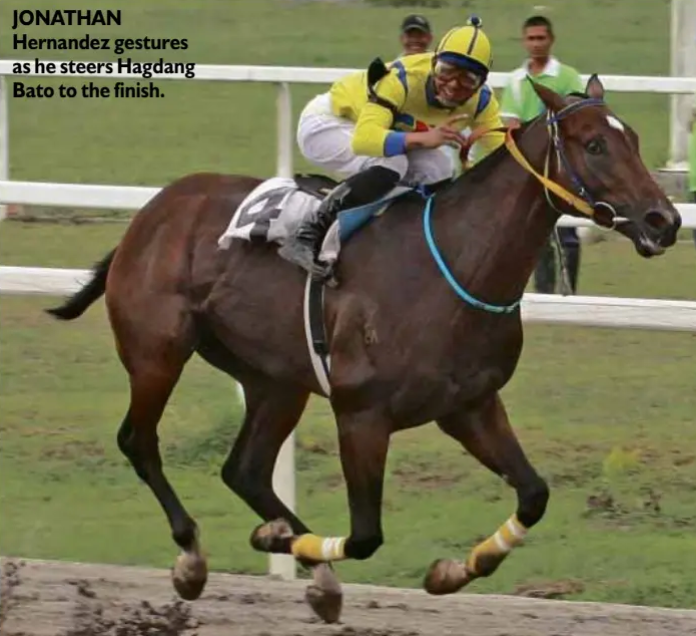
\includegraphics[width=0.4\linewidth]{img/hagdang-bato.png}

    \textit{2012 Philippine Triple Crown winner \textup{Hagdang Bato}, with his jockey JB Hernandez.}

    \textit{Image taken from the Philippine Daily Inquirer}
\end{center}

Cindy is addicted to a brand new horse-racing \textit{gacha} mobile game. The game is a \textit{raising simulator}, meaning the main gameplay loop is the process of training a character.  In this game, each of your characters is a \textit{kabayo}.

Each kabayo has $n$ attributes called ``stats'', each with some positive integer value.  There exists a \textit{stat cap} of $c$, meaning $c$ is the maximum value that any stat can be.

When one playthrough of the game is completed, Cindy's kabayo is assigned a numerical rating that is computed based on its stats, the higher the better.  

However, the rating formula is not linear.  The rating is computed as the \textit{sum of the squares} of each of Alice's kabayo's stats.  For example, with $n=5$, a kabayo with stats $[3, 1, 4, 1, 5]$ would have a rating of
\begin{align*}
    3^2 + 1^2 + 4^2 + 1^2 + 5^2 &= 52.
\end{align*}
Cindy's kabayo begins with some initial stats.  She then will decide how to train her kabayo, meaning she may do the following action at most $k$ times:
\begin{itemize}
    \item Choose one of her kabayo's stats with a value strictly less than $c$; \newline increase its value by $+1$.
\end{itemize}
You are given the initial stats of Cindy's kabayo, as well as $c$ and $k$.  If she raises her kabayo optimally, what is the maximum possible rating she can get?

\subsection*{Input Format}

Input begins with a single line containing the space-separated integers $n$ and $c$ and $k$.

The second line of input contains $n$ space-separated integers, the initial values of Cindy's kabayo's stats.

\subsection*{Output Format}

Output a line containing a single integer, the maximum possible rating.

\subsection*{Constraints}

\textit{Your program will only be tested on data that satisfies the following constraints.}

% Set to (2e5, 1e9, 1e6) in true bounds
\constraints{
    $1 \leq n \leq 100$ \\
    $1 \leq k \leq 2000$ \\
    $1 \leq c \leq 1200$ \\
    $1 \leq \text{each initial stat} \leq c$ \\
}

\textit{There is no need to validate in your program that these constraints hold.}

\subsection*{Sample I/O}

\begin{sampleIO}
\begin{verbatim}
5 6 2
3 1 4 1 5
\end{verbatim}
&
\begin{verbatim}
72
\end{verbatim}
\end{sampleIO}

\begin{sampleIO}
\begin{verbatim}
5 6 1
3 1 4 1 5
\end{verbatim}
&
\begin{verbatim}
63
\end{verbatim}
\end{sampleIO}

\begin{sampleIO}
\begin{verbatim}
5 5 1
3 1 4 1 5
\end{verbatim}
&
\begin{verbatim}
61
\end{verbatim}
\end{sampleIO}

\begin{sampleIO}
\begin{verbatim}
1 1200 99
1
\end{verbatim}
&
\begin{verbatim}
10000
\end{verbatim}
\end{sampleIO}

% \subsection*{Explanation}
